%Cloud-Computing Basics a Non tech. intro.
%Seite 163
% Wie werden die Informationen die Benutzer gezeigt und wie können sie diese manipulieren

Die mit den Überwachungswerkzeuge gesammelte Informationen, bilden die Grundlage für die Optimierungsmaßnahmen.[HIER KONKRETER WERDEN]
In diesem Kapitel werden wir die mit Hilfe der Werkzeuge gesammelten Informationen nutzen, um über die am besten geeigneten Optimierungsmaßnahmen zu entscheiden.

\subsection{Auto Scaling}% Group }
%t.ly/CXs3 Linked In auf DE
%t.ly/1nka
%THIS!!! t.ly/vrCO
%https://youtu.be/qYHR_V1lvNU?t=900
Auto Scaling ist es hilfreich, um die richtige Anzahl von EC2 Instanzen zur Verfügung zu haben, um die Anwendungslast dynamisch abzudecken.
\\\\
%https://www.youtube.com/watch?v=yC5nRYS2IYI En Espaniol
%https://docs.aws.amazon.com/autoscaling/ec2/userguide/as-scaling-simple-step.html#policy-creating-asg-console

Die \autoref{fig:AutoSca_Unused_Capacity} zeigt das wechselnde Verhalten einer Beispielanwendung, die vor allem unter der Woche Ressourcen verbraucht. Am Wochenende sinkt die Nachfrage nach Rechnerkapazität auf weniger als 25 \%. 

Die gelben Säulen stellen die tägliche genutzte Rechenkapazität dar.
Die graue Zone entspricht ungenutzte Rechenkapazität. 
%\begin{center}
    %TODO: selbst das Bild zu erzeugen, um eine bessere Qualität zu bekommen
  %  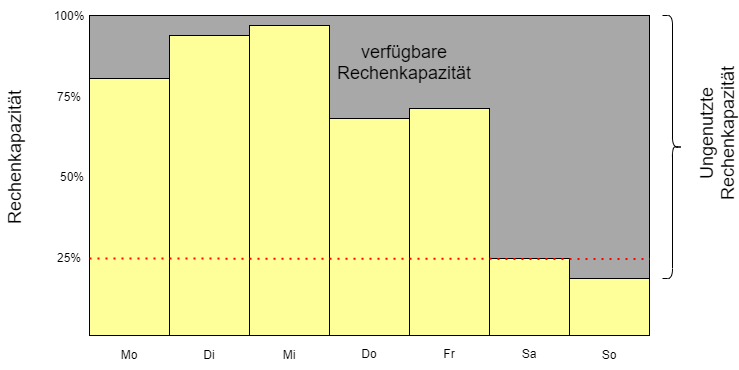
\includegraphics[scale=0.7]{sources/AutoCap Unused Capacity}\label{fig:AutoSca_Unused_Capacity}\\
 %   \textbf{Abbildung \autoref{fig:AutoSca_Unused_Capacity}:} Ungenutzte Ressourcen
  % \footnote{Vgl. u.a.\cite{AMZ01}}
%\end{center}

\begin{figure}[h]
    \centering
    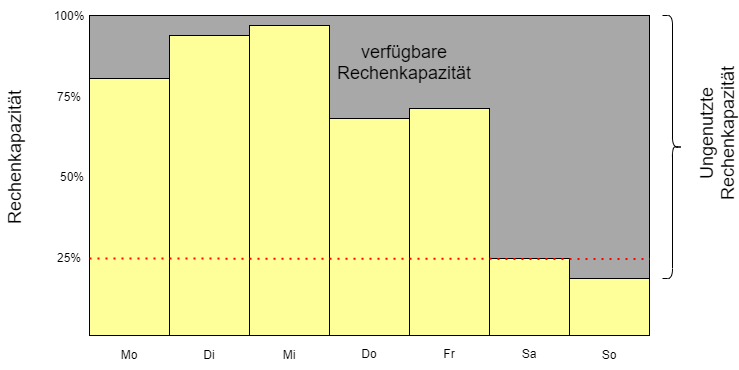
\includegraphics[scale=0.6]{sources/AutoCap Unused Capacity}
    \caption{}\label{fig:AutoSca_Unused_Capacity} Ungenutzte Rechenkapazität. \\
    Quelle: Eigene Darstellung. 
    %\footnote{\cite{AMZ01}}
  \end{figure}

%Zu erklären: cooldown period and scaling policy.


\subsubsection{Zeitgesteuerte Skalierung}
%WE für Dev und Beta
In einem On-Premise-System macht es möglicherweise keinen Unterschied bei den Kosten, wenn die Instanzen aktiv bleiben. 
Im Gegensatz dazu ist es bei On-Demand-Zahlungsmodelle sinnvoll Zeiträume zu definieren, in denen die Instanzen abgeschaltet werden sollen.

Bei Systemen, die nur tagsüber und unter der Woche in Betrieb sein müssen, kann dies eine Einsparung von zu 67\% bedeuten.  Wenn zum Beispiel Test- und Beta-Umgebungen von Montag bis Freitag von 7 bis 20 Uhr laufen.
[DAS WÜRDE IN EUROS GESPART WERDEN: BEISPIEL]
% Automatisiere das Hoch- und Herunterfahren von Instanzen
% https://www.linkedin.com/learning/monitoring-aws-with-cloudwatch/autoscaling-using-alarms?autoAdvance=true&autoSkip=true&autoplay=true&resume=false&u=79182202

% Grund: weil i.d.R., kein Entwickler 24/7 arbeitet.
% Wie?: mit Tagging, Lambda oder mit Auto Scaling Groups.
%Wann ist es sinnvoll Systeme runterzufahren 
%HIER LESEN {\cite{CCB}, Seite 153}


%Weihnachten und BackFriday
Wenn der Zeitpunkt einer großen Nachfrage bekannt ist, kann eine Erhöhung der Rechnerkapazität geplant werden, um Überlastungen zu vermeiden.
Beispiele für solche Zeitpunkte oder Zeiträume sind unter anderem Black-Friday, vor und während Weihnachten und Cyber-Monday.

\subsection{(auto) Tiering }
Grund: nicht alle Dateien brauchen eine hohe Verfügbarkeit.
%Tiering, aber automatisch

\subsection{Automatisierung mit Lambda Funktionen}
Grund: einmal programmiert, funktioniert es für immer.
\\(To-Do:) Möglichkeiten untersuchen, bewerten und die passende Auswählen.

%Limitierung 
%Quotas setzen? erweitern oder reduzieren / benachrichtigen aber auch eine Aktion durchführen 

%Turning stuffs OFF
%Lambda
\begin{comment}
AWS Lambda is a compute service. You can use it to run code without provisioning or managing servers. Lambda runs your code on a high-availability compute infrastructure. It operates and maintains all of the compute resources, including server and operating system maintenance, capacity provisioning and automatic scaling, code monitoring, and logging. With Lambda, you can run code for almost any type of application or backend service. 

Some benefits of using Lambda include the following:

You can run code without provisioning or maintaining servers.
It initiates functions for you in response to events.
It scales automatically.
It provides built-in code monitoring and logging via Amazon CloudWatch.
\end{comment}

%Data Pipeline
%CloudWatch

%Economic Performance?
%QUEUES

%NEVER forget your availability requirements, trying to optimize, first availability THEN cost...
%Do not use your DB for saving BLOB
warum ist das empfehlungswert?

\subsection{VERKAUFE DEINE Ungenutzte Kapazität in RI Marketplace}


%Kombination
%https://spot.io/blog/effective-utilization-of-aws-savings-plans-and-ec2-spot-instances/#a1
%https://www.youtube.com/watch?v=X_7pnzPlESs

 